\section{Билет 6. Формула Кирхгофа решения задачи Коши для неоднородного волнового уравнения в $\R^3$. Метод Дюамеля. Принцип Гюйгенса}
% Иваныч техал
\subsection{Формулировка задачи}

\begin{equation} \label{6_1}
    \begin{cases}
        u_{tt} - a^2\Delta u = f(t, x) & t > 0, x \in \R^3 \\
        \while{u}{t=0} = 0 & \\
        \while{u_t}{t=0} = 0
    \end{cases} \;\;\text{ считаем что } D_x^\alpha f(t, x) \in \C\{t \geq 0, x \in \R^3\} \forall \alpha: \abs{\alpha} \leq 2
\end{equation}

\subsection{Метод Дюамеля}

Сведем задачу к задаче Коши для однородного волнового уравнения. Рассмотрим однопараметрическое семейство задач:
\begin{equation} \label{6_2}
\begin{cases}
    w_{tt}(t, x, \tau) - a^2\Delta_x w(t, x, \tau) = 0 & t > \tau, x \in \R^3 \\
    \while{w}{t=\tau} = 0 & \\
    \while{w_t}{t=\tau} = f(\tau, x) &
\end{cases} \;\;\; \tau \geq 0
\end{equation}


Решение получаем по формуле Пуассона-Кирхгофа:

\begin{equation*}
    w(t, x, \tau) = \frac{1}{4\pi a^2(t - \tau)}\iint_{\abs{\xi - x}=a(t-\tau)}f(\tau, \xi)\;dS_\xi \in \C^2\{t \geq \tau, x \in \R^3\}
\end{equation*}
Введем в рассмотрение функцию
$$
\omega_f(t, x, \tau) = \frac{1}{4\pi a^2t}\iint_{\abs{\xi - x}=at}f(\tau, \xi)\;dS_\xi
$$
Тогда $D^\alpha_{t, x}\omega_f(t, x, \tau)\in \C\{x \in \R^3, t \geq \tau, \tau \geq 0\} \forall \alpha: |\alpha| \leq 2$. 

$$w(t, x, \tau) = \omega_f(t-\tau, x, \tau) \Rightarrow D^\alpha_{t, x}w(t, x, \tau) \in \C\{x \in \R^3, t \geq 0, \tau \geq 0\} \forall \alpha: |\alpha| \leq 2$$

\begin{statement}
    $$
    u(t, x) = \int_0^t w(t, x, \tau)d\tau \text{ --- классическое решение задачи \ref{6_1}}
    $$
\end{statement}
\begin{proof}
\begin{itemize}
    \item $$D^\alpha_{t, x} u(t, x) \in \C\{x \in \R^3, t \geq 0\} \forall \alpha: |\alpha| \leq 2$$
    \item $$\while{u}{t=0} = 0; \;\; \while{u_t}{t=0} = 
    \while{\brs{\underbrace{w(t, x, t)}_{=0 \text{ из условий Коши в \ref{6_2}}} +\int_0^t \pd{w}{t}d\tau}}{t=0} = \while{\int_0^0\pd{w}{t}d\tau}{t=0} = 0$$
    \item $$
    \Delta_xu = \int_0^t\Delta_x w(t, x, \tau)d\tau; \; $$$$ \; u_{tt} = \pd{}{t}\int_0^t \pd{w}{t}\;d\tau = w_t(t, x, t) + \int_0^t w_{tt} (t, x, \tau)\;d\tau = f(t, x) + a^2\int_0^t\Delta_x w(t, x, \tau) \;d\tau = $$
    $$ = f(t, x) + a^2\Delta_x u
    $$
\end{itemize}

Значит, рассматриваемая функция удовлетворяет уравнению.
\end{proof}
Мы доказали следующую теорему:
\begin{theorem}
    Пусть в \ref{6_1} функция $f(t, x): D^\alpha_x f(t, x) \in \C\{t \geq 0, x \in \R^3\}$. Тогда функция 
    \begin{equation} \label{6_3}
        u(t, x) = \int_0^t \frac{1}{4\pi a^2(t - \tau)}\sbrs{\iint_{\abs{\xi - x} = a(t - \tau)}f(\tau, \xi)\;dS_\xi}d\tau
    \end{equation}
    является классическим решением, причем 
    $$
    D^\alpha_{t, x} \in \C\{t \geq 0, x \in \R^3\}
    $$
\end{theorem}
Суть метода Дюамеля: $f(t, x)$ --- это начальные данные в каждый момент времени.

\subsection{Запаздывающий потенциал}
Преобразуем полученную формулу \ref{6_3}. 

\begin{align*}
    \int_0^t \frac{1}{4\pi a^2(t - \tau)}\sbrs{\iint_{\abs{\xi - x} = a(t - \tau)}f(\tau, \xi)\;dS_\xi}d\tau = 
    \begin{bmatrix} a(t - \tau) = \rho \\ \tau = t -\rho/a \\ d\tau = -d\rho/a\end{bmatrix} = -\int_{at}^0\frac{1}{4\pi a \rho}\frac{d\rho}{a}\iint_{\abs{\xi - x} = \rho} f(t - \rho/a, \xi) \;dS_\xi = \\
    = \frac{1}{4\pi a^2}\int_0^{at}\sbrs{\iint_{\abs{\xi - x} = \rho} \frac{f(t - \frac{\abs{\xi - x}}{a}, \xi)}{\abs{\xi - x}}\;dS_\xi}\;d\rho = \boxed{\frac{1}{4\pi a^2} \iiint_{\abs{\xi - x} < at}\frac{f(t - \frac{\abs{\xi - x}}{a}, \xi)}{\abs{\xi - x}}\;d\xi}
\end{align*}

Последнее выражение называется \emph{запаздывающим потенциалом}.

\subsection{Общая задача}
$$
\begin{cases}
    u_{tt} - a^2\Delta_x u = f(t, x) \\
    \while{u}{t=0} = u_0(x) \\
    \while{u_t}{t=0} = u_1(x)
\end{cases}
$$

\begin{theorem}
    Пусть в общей задаче Коши имеем:
    $$
    u_0 \in \C^3(\R), u_1\in \C^2(\R), D^\alpha_{x}f(t, x)\in \C\{t \geq 0, x \in \R^3\} \forall \alpha: \abs{\alpha} \leq 2
    $$
    Тогда 
    \begin{equation} \label{6_4}
        u(t, x) = \pd{}{t}\sbrs{\frac{1}{4\pi a^2t}\iint_{\abs{\xi - x}=at}u_0(\xi)\;dS_\xi} + \frac{1}{4\pi a^2t} \iint_{\abs{\xi - x}=at}u_1(\xi)\;dS_\xi +
        \frac{1}{4\pi a^2} \iiint_{\abs{\xi - x} < at}\frac{f(t - \frac{\abs{\xi - x}}{a}, \xi)}{\abs{\xi - x}}\;d\xi, 
%        
        u(t, x) \in \C^2\{t \ge 0, x \in \R^3\}
    \end{equation}
    является классическим решением общей задачи Коши. Формула \ref{6_4} называется формулой Кирхгофа.
\end{theorem}
\subsection{Принцип Гюйгенса}

Пусть $f=0$, то есть источников нет, а начальное возмущение локализовано в пространстве (носители функций $u_0$ и $u_1$ содержатся в некотором компакте $M$). Тогда в каждой точке воздействие будет локализовано во времени. У такого конечного возмущения есть передний и задний фронты. 
\begin{statement}[Принцип Гюйгенса]
    Возмущение, локализованное в пространстве, приводит к действию, локализованному во времени
\end{statement}

\begin{proof}
Из формулы \hyperref[6_4]{Кирхгофа} видно, что в заданной точке $x_0 \in \R^3$ вне отрезка времени $[t_1; t_2]$ функция
$u(x_0, t)$ тождественна нулю, где 
$$
t_1 = \frac{1}{a}\inf_{y\in M}|y-x_0|, 
~ t_2 = \frac{1}{a} \sup_{y \in M}|y-x_0|
$$
\end{proof}

\begin{center}
    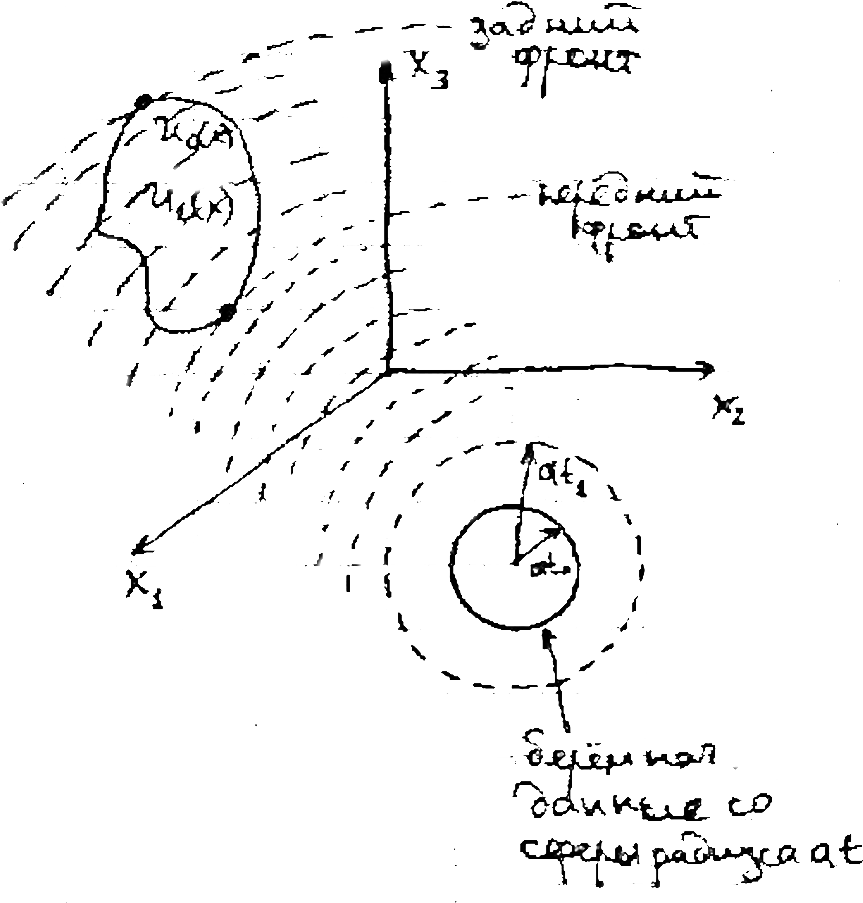
\includegraphics[width=0.4\textwidth]{6_1_new}
\end{center}
